% =========================================
% Figure — Board Anatomy (Diamond)
% Homes: (1,8) & (8,1)   Sanctums: (8,8) & (1,1)
% (Opposite corners are Homes; the other two corners are Sanctums)
% If you drive Sanctums via macros, set:
% \renewcommand{\SanctumA}{8/8}   % one Sanctum corner
% \renewcommand{\SanctumB}{1/1}   % the other Sanctum corner
% =========================================

\begin{figure}[H]
  \centering
  \begin{tikzpicture}[x=0.6cm,y=0.6cm]
    \newcommand{\yphys}[1]{\numexpr\BoardN-#1\relax}

    \begin{scope}[rotate around={45:(4,4)}]
      % Base grid + center shading
      \DrawGrid
      \ShadeCross{cross}

      % --- Corner assignment (rotated roles) ---
      % Homes (two opposite corners):
      \ShadeSquares{apexA}{1/8}   % Home
      \ShadeSquares{apexB}{8/1}   % Home

      % Sanctums (the remaining two corners):
      \ShadeSquares{sanctumA}{8/8}  % Sanctum
      \ShadeSquares{sanctumB}{1/1}  % Sanctum

      % Crisp borders back on top
      \RedrawGridLines

      % Upright labels (no directional words)
      \node[font=\scriptsize, fill=white, inner sep=1pt, transform shape=false]
        at ({1-0.5},{\yphys{8}+0.5}) {Home Apex};

      \node[font=\scriptsize, fill=white, inner sep=1pt, transform shape=false]
        at ({8-0.5},{\yphys{1}+0.5}) {Home Apex};

      \node[font=\scriptsize, fill=white, inner sep=1pt, transform shape=false]
        at ({8-0.5},{\yphys{8}+0.5}) {Sanctum};

      \node[font=\scriptsize, fill=white, inner sep=1pt, transform shape=false]
        at ({1-0.5},{\yphys{1}+0.5}) {Sanctum};

      % Central Four label
      \draw[decorate,decoration={brace,amplitude=3pt},blue!60] (3,5.05) -- (5,5.05);
      \node[font=\scriptsize, blue!60, transform shape=false, anchor=south]
        at (4,5.25) {Central Four};
    \end{scope}
  \end{tikzpicture}
  \caption{Diamond orientation with opposite Homes and the remaining corners as Sanctums (roles rotated 90°).}
  \label{fig:board-anatomy-rot90}
\end{figure}

% =========================================
% Figure — Movement Lanes (Onward / Homeward)
% Lane labels placed at the arrow TIPS (slightly offset for clarity)
% =========================================
\begin{figure}[H]
  \centering

  % --- Left: Onward lanes (OnL / OnR) ---
  \begin{minipage}[t]{0.47\linewidth}
    \centering
    \begin{tikzpicture}[x=0.55cm,y=0.55cm]
      \begin{scope}[rotate around={45:(4,4)}]
        \DrawGrid
        \ShadeCross{cross}
        \RedrawGridLines

        \coordinate (Q) at (4.5,4.5);

        % OnL: from center to +x (appears up-right)
        \draw[moveArrow, draw=ccol, line cap=round] (Q) -- ++(2,0);
        % Tip label (slight outwards offset)
        \node[font=\scriptsize, fill=white, inner sep=1pt]
          at ($(Q)+(2,0)+(0.22,0.22)$) {OnL};

        % OnR: from center to +y (appears up-left)
        \draw[moveArrow, draw=scol, line cap=round] (Q) -- ++(0,2);
        % Tip label (slight outwards offset)
        \node[font=\scriptsize, fill=white, inner sep=1pt]
          at ($(Q)+(0,2)+(-0.22,0.22)$) {OnR};

        % Origin dot
        \fill[black] (Q) circle[radius=0.05];

        % Legend at the TOP
        \node[fill=white, inner sep=2pt, font=\scriptsize, anchor=north east]
          at (7.7,7.7) {Onward exact: R=2,\ O=3,\ G=4,\ B=5};
      \end{scope}
    \end{tikzpicture}
    \par\smallskip
    \scriptsize Onward lanes (\texttt{OnL}, \texttt{OnR}) — exact step counts
  \end{minipage}
  \hfill
  % --- Right: Homeward lanes (HmL / HmR) ---
  \begin{minipage}[t]{0.47\linewidth}
    \centering
    \begin{tikzpicture}[x=0.55cm,y=0.55cm]
      \begin{scope}[rotate around={45:(4,4)}]
        \DrawGrid
        \ShadeCross{cross}
        \RedrawGridLines

        \coordinate (Q) at (4.5,4.5);

        % HmL: from center to -x (appears down-left)
        \draw[moveArrow, draw=rocol, line cap=round] (Q) -- ++(-2,0);
        % Tip label (slight outwards offset)
        \node[font=\scriptsize, fill=white, inner sep=1pt]
          at ($(Q)+(-2,0)+(-0.22,-0.22)$) {HmL};

        % HmR: from center to -y (appears down-right)
        \draw[moveArrow, draw=rccol, line cap=round] (Q) -- ++(0,-2);
        % Tip label (slight outwards offset)
        \node[font=\scriptsize, fill=white, inner sep=1pt]
          at ($(Q)+(0,-2)+(0.22,-0.22)$) {HmR};

        % Origin dot
        \fill[black] (Q) circle[radius=0.05];

        % Legend lower-right (nudged to avoid overlap)
        \node[fill=white, inner sep=2pt, font=\scriptsize, anchor=north east]
          at (7.55,6.75) {Homeward up to:\ R$\le1$, O$\le2$, G$\le3$, B$\le4$};
      \end{scope}
    \end{tikzpicture}
    \par\smallskip
    \scriptsize Homeward lanes (\texttt{HmL}, \texttt{HmR}) — “up to” step counts
  \end{minipage}

  \caption{Movement lanes from a square center. Arrows cross grid lines at midpoints for unambiguous pathing.}
  \label{fig:lanes}
\end{figure}

% =========================================
% [3] Figure — ZoC: Entering Stops the Move
% Shows a legal entry into enemy ZoC and that you cannot pass through it
% =========================================
\begin{figure}[H]
  \centering
  \begin{tikzpicture}[x=0.6cm,y=0.6cm]
    \begin{scope}[rotate around={45:(4,4)}]
      \DrawGrid
      \ShadeCross{cross}
      \RedrawGridLines

      % Enemy piece at (5,4); shade its ZoC (4/4,6/4,5/3,5/5)
      \ShadeSquares{zoc}{4/4,6/4,5/3,5/5}
      \PlaceB{R}{5}{4}

      % Our Blue starts at (2,4), intends to slide rightward (to 4/4)
      % Centers: (2,4)->(1.5,4.5), (4,4)->(3.5,4.5), (6,4)->(5.5,4.5)
      \draw[moveArrow,draw=royal!85!black,line cap=round]
        (1.5,4.5) -- (3.5,4.5);

      % Dashed "would-be continuation" (illegal; entering ZoC stops move)
      \draw[moveArrow,draw=royal!50!black,dashed,line cap=round]
        (3.5,4.5) -- (5.5,4.5);

      % Blue piece at start square
      \PlaceA{B}{2}{4}

      % Callout: Enter ZoC — stop
      \node[font=\scriptsize,fill=white,inner sep=1pt,anchor=north]
        at (3.5,4.3) {Enter enemy ZoC $\Rightarrow$ \emph{move ends}};
      \node[font=\scriptsize,fill=white,inner sep=1pt,anchor=south]
        at (5.5,4.7) {\emph{no pass-through}};

      % A small "X" to mark the illegal continuation end
      \node[font=\bfseries\footnotesize, text=red!70!black] at (5.5,4.5) {$\times$};
    \end{scope}
  \end{tikzpicture}

  \caption{Entering enemy ZoC is legal but \emph{ends the move}; you cannot continue the slide through ZoC.}
  \label{fig:zoc-stop}
\end{figure}

% =========================================
% [4] Figure — Blue Specials: Hop vs. Displacement (before/after)
% Enemy is an Orange (O), placed away from the Central Four (y=6)
% =========================================
\begin{figure}[H]
  \centering

  % -------- Hop-capture --------
  \begin{subfigure}[t]{0.48\linewidth}
    \centering
    % BEFORE (left mini)
    \begin{tikzpicture}[x=0.52cm,y=0.52cm]
      \begin{scope}[rotate around={45:(4,4)}]
        \DrawGrid
        \ShadeCross{cross}
        \RedrawGridLines

        % Blue at (3,6); enemy Orange at (4,6); landing (5,6) is empty
        % Centers (unrotated coords, then drawn inside rotated scope):
        % (3,6)->(2.5,2.5), (4,6)->(3.5,2.5), (5,6)->(4.5,2.5)
        \PlaceA{B}{3}{6}
        \PlaceB{O}{4}{6}

        % Hop arrow: from Blue over enemy to empty beyond
        \draw[moveArrow,draw=royal!85!black,line cap=round]
          (2.5,2.5) .. controls (3.0,2.5) .. (4.5,2.5);

        \node[font=\scriptsize,fill=white,inner sep=1pt,anchor=south]
          at (3.5,2.7) {Hop over};
      \end{scope}
    \end{tikzpicture}
    \hspace{6pt}
    % AFTER (right mini)
    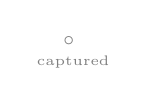
\begin{tikzpicture}[x=0.52cm,y=0.52cm]
      \begin{scope}[rotate around={45:(4,4)}]
        \DrawGrid
        \ShadeCross{cross}
        \RedrawGridLines

        % After hop: Blue now at (5,6); enemy removed
        \PlaceA{B}{5}{6}

        % Ghost mark where enemy was (optional visual aid)
        \node[font=\scriptsize, text=black!50] at (3.5,2.5) {$\circ$};
        \node[font=\tiny, text=black!50,anchor=north] at (3.5,2.35) {captured};
      \end{scope}
    \end{tikzpicture}

    \caption{Hop-capture (jump over 1 adjacent enemy to the empty square beyond; remove the jumped piece).}
  \end{subfigure}
  \hfill
  % -------- Displacement --------
  \begin{subfigure}[t]{0.48\linewidth}
    \centering
    % BEFORE (left mini)
    \begin{tikzpicture}[x=0.52cm,y=0.52cm]
      \begin{scope}[rotate around={45:(4,4)}]
        \DrawGrid
        \ShadeCross{cross}
        \RedrawGridLines

        % Blue at (3,6); enemy Orange at (4,6)
        \PlaceA{B}{3}{6}
        \PlaceB{O}{4}{6}

        % Displacement arrow: step onto adjacent enemy
        \draw[moveArrow,draw=royal!85!black,line cap=round]
          (2.5,2.5) -- (3.5,2.5);

        \node[font=\scriptsize,fill=white,inner sep=1pt,anchor=south]
          at (3.0,2.7) {Displace};
      \end{scope}
    \end{tikzpicture}
    \hspace{6pt}
    % AFTER (right mini)
    \begin{tikzpicture}[x=0.52cm,y=0.52cm]
      \begin{scope}[rotate around={45:(4,4)}]
        \DrawGrid
        \ShadeCross{cross}
        \RedrawGridLines

        % After displacement: Blue at (4,6); enemy removed
        \PlaceA{B}{4}{6}

        % Ghost mark where Blue came from (optional)
        \node[font=\scriptsize, text=black!50] at (2.5,2.5) {$\circ$};
        \node[font=\tiny, text=black!50,anchor=north] at (2.5,2.35) {from};
      \end{scope}
    \end{tikzpicture}

    \caption{Displacement (step onto an adjacent enemy square; remove it).}
  \end{subfigure}

  \vspace{4pt}
  {\footnotesize\itshape
   One special per Blue turn. Slide→special is legal \emph{unless} the slide entered enemy ZoC (entering ZoC ends the move). No special→slide.}

  \caption{Blue specials (before/after), demonstrated away from the Central Four.}
  \label{fig:blue-specials}
\end{figure}

% =========================================
% [6] Figure — Twin Apex Seed + Mobilization Delay (worked examples)
% Panels: (a) Slide→Seed→Rooted. (b) Reforge→Sanctum, later Seed from other Sanctum.
% Sanctums at (8,8) and (1,1) to match earlier anatomy figure.
% =========================================
\begin{figure}[H]
  \centering

  % ---------- (a) Slide → Seed → Rooted ----------
  \begin{subfigure}[t]{0.48\linewidth}
    \centering
    % BEFORE: slide to Sanctum
    \begin{tikzpicture}[x=0.52cm,y=0.52cm]
      \begin{scope}[rotate around={45:(4,4)}]
        \DrawGrid
        \ShadeCross{cross}
        % Shade Sanctums for clarity
        \ShadeSquares{sanctumA}{8/8}
        \ShadeSquares{sanctumB}{1/1}
        \RedrawGridLines

        % Blue starts near top-right, slides onto (8,8)
        \PlaceA{B}{7}{7}
        \draw[moveArrow,draw=royal!85!black,line cap=round]
          (6.5,1.5) -- (7.5,0.5); % to (8,8) center
        \node[font=\scriptsize,fill=white,inner sep=1pt,anchor=west]
          at (7.55,0.55) {slide to Sanctum};
      \end{scope}
    \end{tikzpicture}
    \hspace{6pt}
    % AFTER: Seed to opposite Sanctum; Blue becomes Rooted
    \begin{tikzpicture}[x=0.52cm,y=0.52cm]
      \begin{scope}[rotate around={45:(4,4)}]
        \DrawGrid
        \ShadeCross{cross}
        \ShadeSquares{sanctumA}{8/8}
        \ShadeSquares{sanctumB}{1/1}
        \RedrawGridLines

        % Blue remains on (8,8), Green spawns at (1,1)
        \PlaceA{B}{8}{8}
        \PlaceA{G}{1}{1}

        % Dashed "Seed" arc for visual link
        \draw[royal!70!black, dashed, -{Latex[length=2.5mm]}]
          (7.5,0.5) .. controls (6.0,2.0) and (2.0,6.0) .. (0.5,7.5);

        % Rooted tag near Blue
        \node[font=\scriptsize,fill=white,inner sep=1pt,anchor=south east]
          at (7.6,0.9) {Rooted};
      \end{scope}
    \end{tikzpicture}

    \caption{Slide onto a Sanctum, then \emph{Seed} to the opposite Sanctum (if empty and cap\,$<\!6$); the Blue becomes \textbf{Rooted} until your next turn.}
  \end{subfigure}
  \hfill
  % ---------- (b) Reforge → Sanctum; later Seed from the other Sanctum ----------
  \begin{subfigure}[t]{0.48\linewidth}
    \centering
    % STEP 1: Reforge places on a Sanctum (no same-Sanctum Seed)
    
\begin{tikzpicture}[x=0.52cm,y=0.52cm]
      \begin{scope}[rotate around={45:(4,4)}]
        \DrawGrid
        \ShadeCross{cross}
        \ShadeSquares{sanctumA}{8/8}
        \ShadeSquares{sanctumB}{1/1}
        \RedrawGridLines

        \PlaceA{B}{8}{8}

        % Small badge noting Reforge placement & same-Sanctum ban
        \node[font=\scriptsize,fill=white,inner sep=1pt,anchor=north east,align=right]
          at (7.8,0.2) {\textsc{Reforge}\\no Seed here};
      \end{scope}
    \end{tikzpicture}
    \hspace{6pt}
    % STEP 2: Later, Blue reaches the other Sanctum and Seeds back
    \begin{tikzpicture}[x=0.52cm,y=0.52cm]
      \begin{scope}[rotate around={45:(4,4)}]
        \DrawGrid
        \ShadeCross{cross}
        \ShadeSquares{sanctumA}{8/8}
        \ShadeSquares{sanctumB}{1/1}
        \RedrawGridLines

        % Blue at (1,1), Seed spawns Green at (8,8)
        \PlaceA{B}{1}{1}
        \PlaceA{G}{8}{8}

        % Dashed Seed arc the other way
        \draw[royal!70!black, dashed, -{Latex[length=2.5mm]}]
          (0.5,7.5) .. controls (2.0,6.0) and (6.0,2.0) .. (7.5,0.5);

        \node[font=\scriptsize,fill=white,inner sep=1pt,anchor=south west,align=left]
          at (0.2,7.8) {Seed allowed\\(different Sanctum)};
      \end{scope}
    \end{tikzpicture}

    \caption{A Blue \emph{placed by Reforge} onto a Sanctum may \textbf{not} Seed from that same Sanctum; later Seeding from the \emph{other} Sanctum is legal. Reforge placement is \emph{not} a “departure from Home” for Mobilization.}
  \end{subfigure}

  \caption{Twin Apex Seed and Mobilization delay: (a) Slide→Seed→Rooted; (b) Reforge→Sanctum, then a later Seed from the opposite Sanctum (same-Sanctum Seed banned).}
  \label{fig:seed-mobilize}
\end{figure}

% =========================================
% [5] Figure — Cross Timers: 3-Stay / 2-Exclusion (7-row timeline)
% Fix: exclusion bands drawn on BACKGROUND layer, under text.
% Requires: \usetikzlibrary{decorations.pathreplacing,arrows.meta,backgrounds}
% =========================================
\begin{figure}[H]
  \centering
  \begin{tikzpicture}[x=1cm,y=0.9cm]
    % Row Y positions (top to bottom)
    \def\yAone{7}
    \def\yBone{6}
    \def\yAtwo{5}
    \def\yBtwo{4}
    \def\yAthree{3}
    \def\yBthree{2}
    \def\yAfour{1}

    % Faint row guides
    \foreach \y in {\yAone,\yBone,\yAtwo,\yBtwo,\yAthree,\yBthree,\yAfour}{
      \draw[black!10] (0.2,\y+0.35) -- (8.6,\y+0.35);
      \draw[black!10] (0.2,\y-0.35) -- (8.6,\y-0.35);
    }

    % === Background shading for exclusion rows (A3 & A4) ===
    % Only under the "Cross timer" + "Notes" columns so text isn't obscured.
    \begin{scope}[on background layer]
      \fill[rccol!12] (3.05,\yAthree+0.38) rectangle (8.55,\yAthree-0.38);
      \fill[rccol!12] (3.05,\yAfour+0.38)  rectangle (8.55,\yAfour-0.38);
    \end{scope}

    % Column headers
    \node[font=\scriptsize\bfseries,anchor=west] at (0.35,\yAone+0.7) {End square};
    \node[font=\scriptsize\bfseries,anchor=west] at (3.20,\yAone+0.7) {Cross timer};
    \node[font=\scriptsize\bfseries,anchor=west] at (6.10,\yAone+0.7) {Notes};

    % Left row labels
    \node[anchor=east,font=\footnotesize] at (0,\yAone)   {A1};
    \node[anchor=east,font=\footnotesize] at (0,\yBone)   {B1};
    \node[anchor=east,font=\footnotesize] at (0,\yAtwo)   {A2};
    \node[anchor=east,font=\footnotesize] at (0,\yBtwo)   {B2};
    \node[anchor=east,font=\footnotesize] at (0,\yAthree) {A3};
    \node[anchor=east,font=\footnotesize] at (0,\yBthree) {B3};
    \node[anchor=east,font=\footnotesize] at (0,\yAfour)  {A4};

    % --- Content ---
    % A1 stay 1/3
    \node[font=\scriptsize,anchor=west] at (0.35,\yAone) {in Cross};
    \node[font=\scriptsize,anchor=west,text=royal!80!black] at (3.20,\yAone) {stay 1/3};
    \node[font=\scriptsize,anchor=west] at (6.10,\yAone) {counts only when turn ends inside};

    % B1
    \node[font=\scriptsize,anchor=west] at (0.35,\yBone) {—};
    \node[font=\scriptsize,anchor=west] at (3.20,\yBone) {—};
    \node[font=\scriptsize,anchor=west] at (6.10,\yBone) {opponent turn};

    % A2 stay 2/3
    \node[font=\scriptsize,anchor=west] at (0.35,\yAtwo) {in Cross};
    \node[font=\scriptsize,anchor=west,text=royal!80!black] at (3.20,\yAtwo) {stay 2/3};
    \node[font=\scriptsize,anchor=west] at (6.10,\yAtwo) {must exit before a 4th end-in-Cross};

    % B2
    \node[font=\scriptsize,anchor=west] at (0.35,\yBtwo) {—};
    \node[font=\scriptsize,anchor=west] at (3.20,\yBtwo) {—};
    \node[font=\scriptsize,anchor=west] at (6.10,\yBtwo) {opponent turn};

    % A3 leaves Cross -> exclusion 1/2
    \node[font=\scriptsize,anchor=west] at (0.35,\yAthree) {outside};
    \node[font=\scriptsize,anchor=west,text=rccol!90!black] at (3.20,\yAthree) {exclusion 1/2};
    \node[font=\scriptsize,anchor=west] at (6.10,\yAthree) {re-entry forbidden this turn};

    % B3
    \node[font=\scriptsize,anchor=west] at (0.35,\yBthree) {—};
    \node[font=\scriptsize,anchor=west] at (3.20,\yBthree) {—};
    \node[font=\scriptsize,anchor=west] at (6.10,\yBthree) {opponent turn};

    % A4 exclusion 2/2
    \node[font=\scriptsize,anchor=west] at (0.35,\yAfour) {outside};
    \node[font=\scriptsize,anchor=west,text=rccol!90!black] at (3.20,\yAfour) {exclusion 2/2};
    \node[font=\scriptsize,anchor=west] at (6.10,\yAfour) {may re-enter starting next A turn};

    % Legend
    \node[font=\scriptsize,anchor=west] at (0.35,0.1)
      {Stay increments only when your \emph{turn ends} in the Cross; after you leave, serve two of your turns before re-entry.};
  \end{tikzpicture}

  \caption{Cross timers illustrated over seven plies (A/B/A/…): two counted stays inside the Cross, then exit; the next two A turns are exclusion (no re-entry).}
  \label{fig:cross-timer}
\end{figure}




